\documentclass[../pfc.tex]{subfiles}
	
\begin{document}

	
	\section{Construcción}
	
	Para la implementación en un principio las metodologías ágiles no marcaban ninguna pauta más allá de que todo lo que no está terminado al 100\% no está terminado y por otro lado que siempre hay que entregar con la máxima calidad posible, aunque quizá la más importante fue que la propiedad del código es colectiva, ya no hay más código mio o código tuyo y tenemos responsabilidades y atribuciones sobre nuestras parcelas, el código es del equipo entero y todo miembro puede y debe mejorar el mismo si observa y detecta un error.\\*
	
	Después de un tiempo de maduración de las mismas surgieron técnicas y disciplinas, algunas en el seno de alguna de estas metodologías (XP sobre todo) y algunas se incorporaron rápidamente desde el movimiento Craftmanship software \cite{manifestocraft} que tiene una filosofía similar aunque más cercana y centrada en el proceso de construcción en sí que en el resto del proceso de desarrollo del proyecto o producto. Estas técnicas son Pair Programming, TDD, Code Reviews y algunas centradas en la mejora del equipo en todos los proyectos como puedan ser Code Retreats, Katas, Koans, etc(citas a gogo). todas estas técnicas y disciplinas hoy en día se consideran tan apegadas a las metodologías ágiles que prácticamente se confunden con las mismas cuando hablamos del proceso de implementación.\\*
	
	Lo que si existe es la idea del visual management, o tener algún tipo de respaldo visual del estado de un proyecto. Para esto existen pizarras en las que mediante el uso de tarjetas, imanes, post its, imágenes e incluso avatares de los miembros del equipo. Esto permite que cualquier persona interesada en el proyecto con solamente dar un vistazo a la pizarra vea el estado del sprint actual, en que trabaja cada miembro del equipo, el estado del backlog, las historias completadas, y demás información que cada equipo adapta a sus necesidades. Recordemos que la idea es que el equipo y el product owner se sientan cómodos con la metodología y la adapten a sus necesidades o idiosincrasia, teniendo en cuenta que no hay balas de plata que sirvan para todo y arreglen los problemas de la noche a la mañana.\\* 
	
	Existen también multitud de utilidades de software que permiten esto mismo para equipos remotos o para aquellos que no les es posible disponer de una pizarra física. Esta ha sido la opción utilizada por nosotros a través de la aplicación web Trello.\\*
	
	\begin{figure}[H]
		\centering
		
\includegraphics[width=0.5\linewidth]{../images/TrelloLogo}
		\caption{Logo de la aplicación Trello}
		\label{fig:trello}
	\end{figure}
	
	Esta app permite el uso de la pantalla como si de una pizarra electrónica se tratase. Para nuestro propósito la dividimos en diferentes columnas  que representarán los estados de una historia de usuario y además algunas zonas para colocar una imagen del burndown, el estado de animo del equipo y del product owner.\\*
	
	\begin{figure}[H]
		\centering
		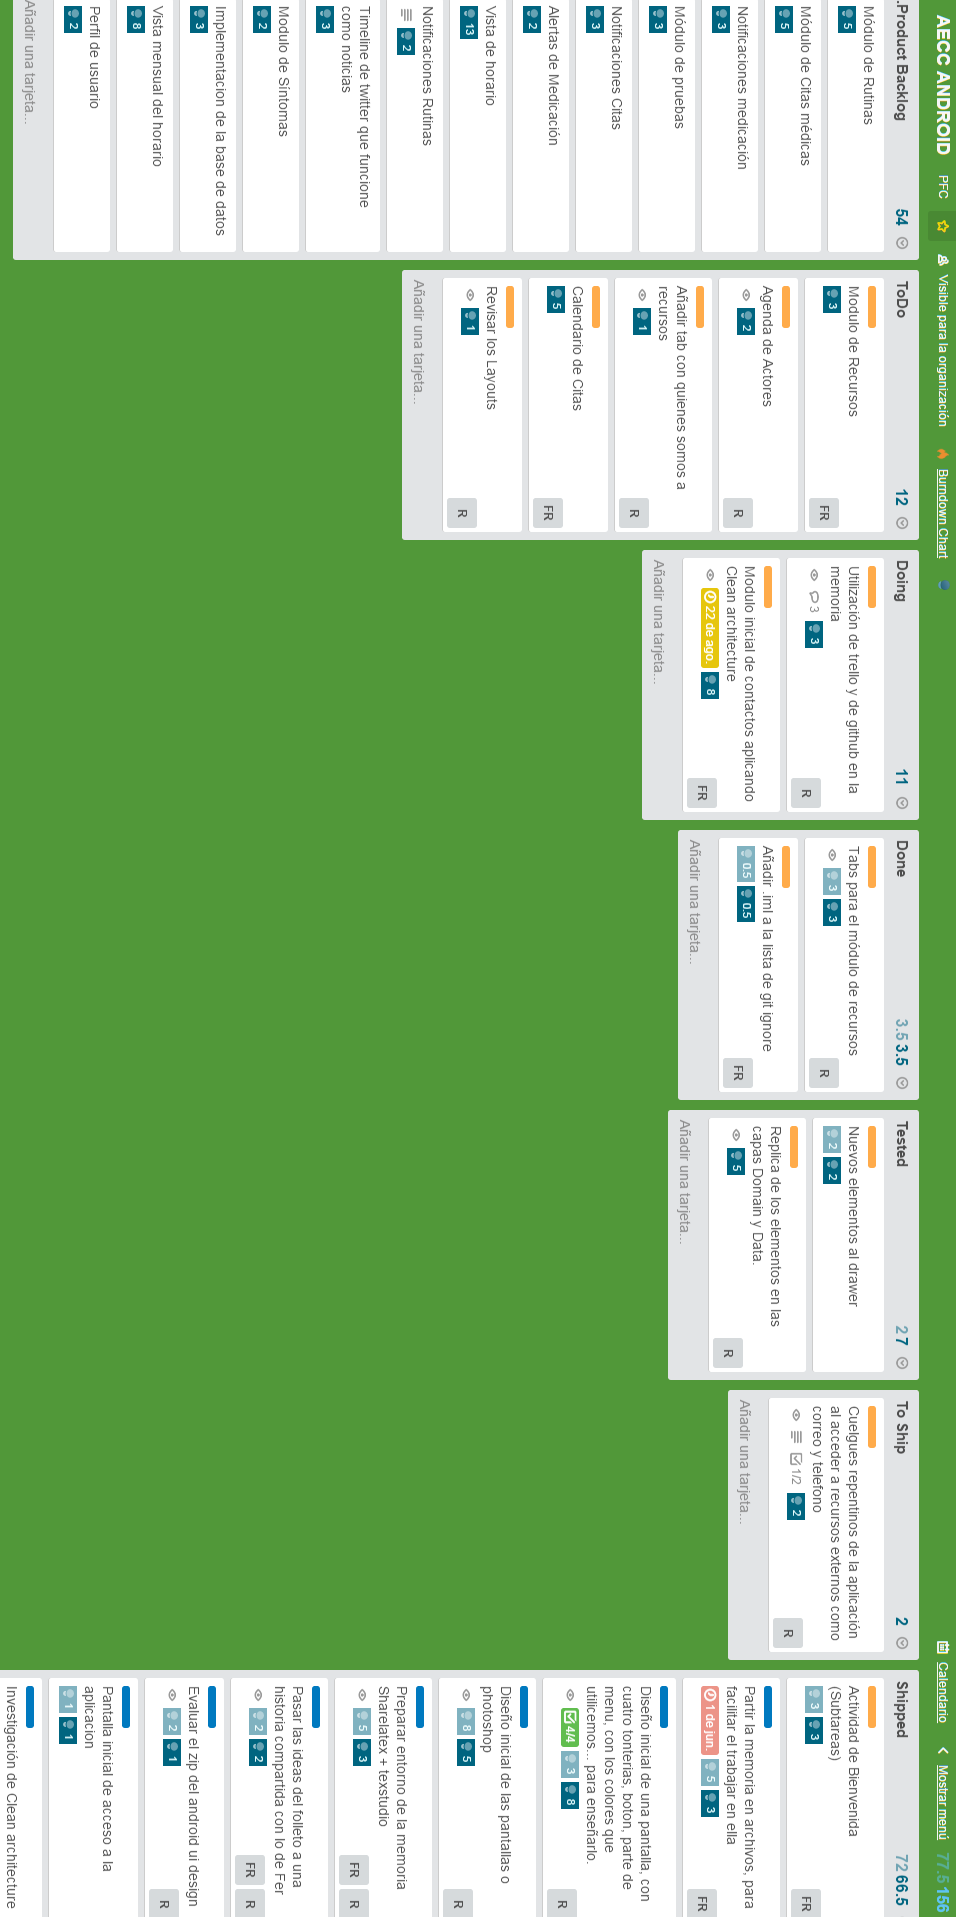
\includegraphics[width=0.8\linewidth]{../images/trello_completo}
		\caption{Trello permite scrum de manera fácil}
		\label{fig:trello}
	\end{figure}
	
	Las columnas que definimos como estados para las historias de usuario fueron:
	
	\begin{itemize} 
		\item Product Backlog es el backlog de la aplicación del que se habló en el Capitulo 3. Debe estar priorizado para que el equipo tenga una visión aproximada de los intereses del product owner en futuros sprints pero, el equipo ha de ser consciente de que esto puede ser modificado por el product owner.
		\item Sprint Backlog o ToDo son las tareas del sprint en curso o por hacer. Pueden estar priorizadas por el product owner para que el equipo tenga cierta idea de lo que es más valioso para el, pero el equipo es libre del orden de implementación de las historias en un sprint. 
		\item Doing es la columna de las historias que actualmente se encuentran en proceso de implementación por algún miembro del equipo.
		\item Done o ToTest tareas que el equipo ha dado por terminadas con sus test unitarios y prueba de aceptación o deinition of done completado, pero no por alguien ajeno al desarrollo de la misma. 
		\item Tested alguien ajeno al desarrollo de la historia de usuario ha testado el criterio de aceptación de la historia, esto puede ser  llevado a cabo por el scrum master o algún miembro del equipo. 
		\item ToShip historias que se han probado por aquieten ajena a quien la desarrolló y pero que aun no han sido entregadas o desplegadas para demo o validación por el product owner.
		\item Shipped historias que fueron entregadas o desplegadas en otros sprints o en una demo, idealmente no deberían salir de esta columna ya que como se dice han sido validadas por el product owner, pero pudiera ser que se presenten errores en test de regresión al añadir nueva funcionalidad. En ese caso pasarían al Product Backlog para el siguiente sprint como historia de defecto, tal y como esté acordado por el equipo.
	\end{itemize}
	
		\begin{figure}[H]
			\centering
			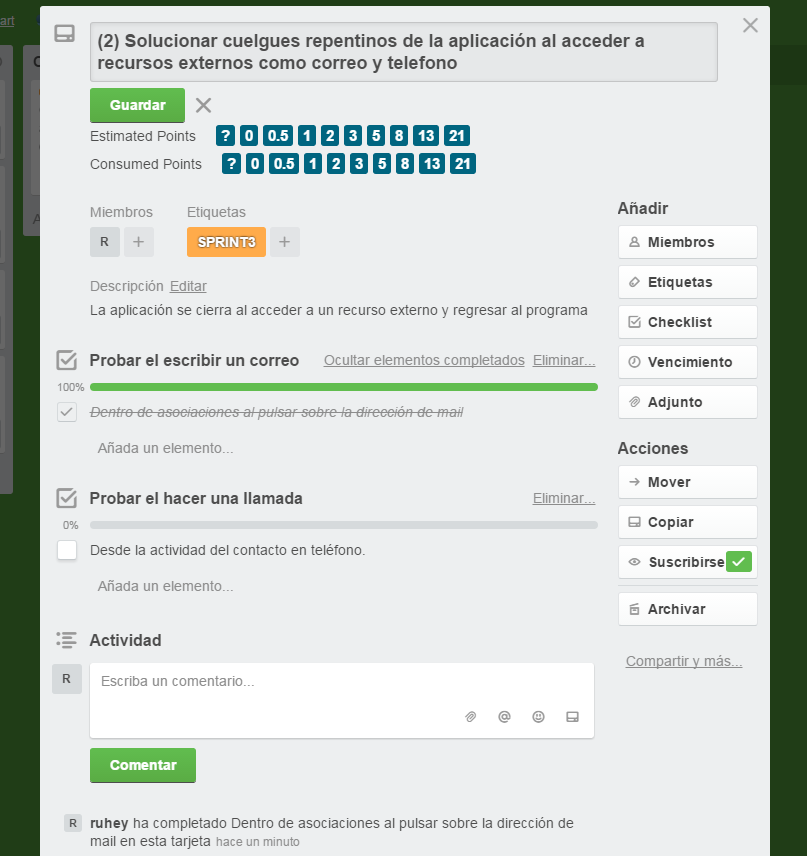
\includegraphics[width=0.7\linewidth]{../images/tarea}
			\caption{Implementación de las Historias de usuario}
			\label{fig:tareaTrello}
		\end{figure}
		
		
		\begin{figure}[H]
			\centering
			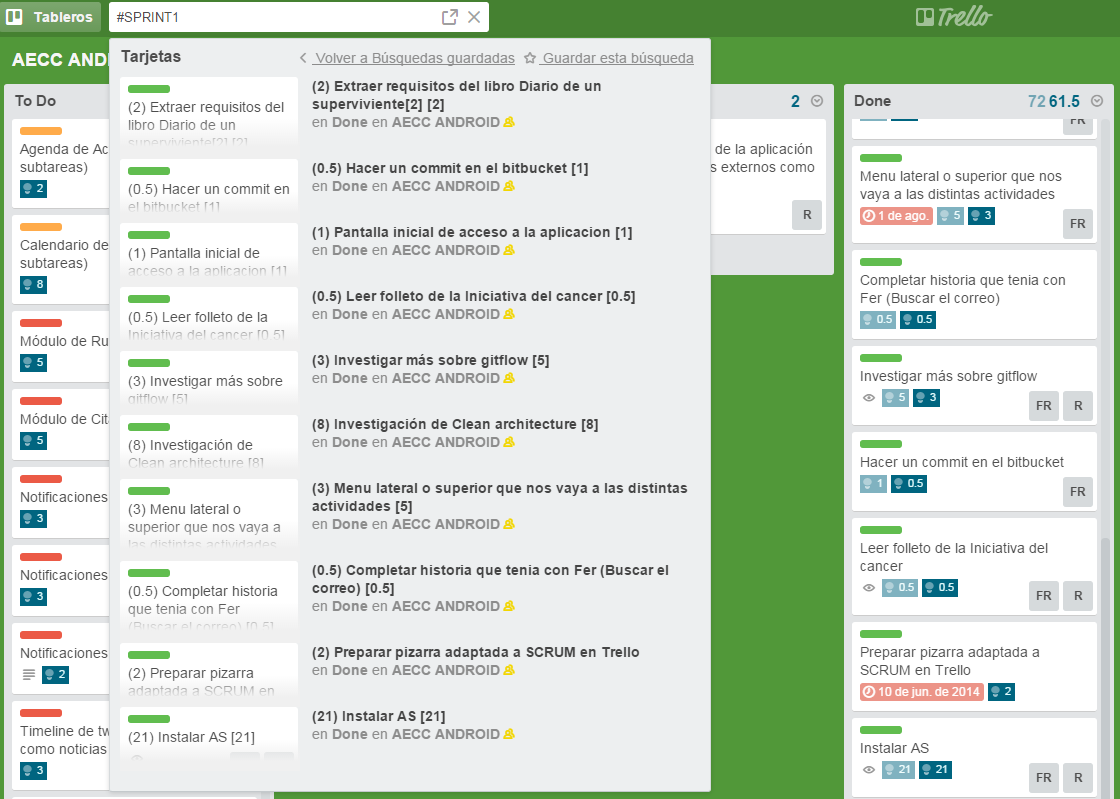
\includegraphics[width=0.7\linewidth]{../images/sprints2}
			\caption{Agrupación de tareas por sprints}
			\label{fig:sprints}
		\end{figure}

	
	\section{Estructura de la aplicación}
	
	\section{Plan de desarrollo}
	Pasos para el desarrollo de la aplicación móvil "Diario de un Superviviente":\\
	
	\textbf{Idea Inicial}
	
	Partimos de la 'idea' conformada junto a la AECC de una aplicación Android  que permitiese a los enfermos de cáncer llevar de una manera mucho mas sencilla el control de las acciones que acontecen de manera rutinaria en su día a día, tales como la toma de medicamentos, asistencia a citas médicas, control de síntomas y pruebas, rutinas diarias beneficiosas.
	
	Para ello la AECC puso a nuestra disposición un folleto que forma parte de esta iniciativa, pero que dadas sus características físicas se que da algo corto en su planteamiento.\\
	
	\textbf{Captura de requisitos}
	
	El proyecto debe estar bien definido, tanto sus objetivos como las funcionalidades que se requieren para que cumpla su cometido. Cuanta mejor definido esté más cerca estaremos de cumplir sus objetivos.
	
	Está tarea, se ha realizado estudiando de manera pormenorizada la documentación que puso a nuestra disposición la AECC dividiendo en partes bien diferenciadas las funcionalidades de cada una de las partes de las que se compone esta documentación.
	
	A través del cruce de correos y de alguna que otra reunión presencial se han limado distintas formas de ver algunas partes.\\
	
		
	Con la definición del proyecto terminada, es necesario saber el tiempo que nos va a llevar en horas, por lo que hay que valorar el desarrollo. Para ello, será necesario contabilizar y estimar los plazos en horas que nos va a costar cada parte del proyecto. Tanto el plazo como el precio dependerán totalmente de las funcionalidades y del tipo de desarrollo elegido, pues no es lo mismo (ni se obtiene un proyecto de igual calidad) desarrollar apps nativas que híbridas, ni que el proyecto requiera de un complejo backend orientado a móviles o no requiera siquiera esta parte.\\
	
	\textbf{Planificación} 
		
	Es la primera fase del desarrollo del proyecto. Consiste en tener un programa de trabajo con un desglose de todas las actividades que se van a realizar (desde el diseño hasta las pruebas finales), el plazo estimado de horas que se le va a dedicar cada una de ellas y estableciendo los medios humanos que se van a dedicar para alcanzar los objetivos que se hayan propuesto. En este proceso, que ha de ser continuo se han de reflejar\\
	
	-Equipos, programas, licencias etc que se vayan a emplear.
	
	-Requerimientos gráficos y fechas límite.
	
	-Necesidades que dependan del cliente (AECC) y fechas para tenerlos disponibles.
	
	-Cambios que puedan ocurrir durante el desarrollo de la app.
	
	Una buena planificación y su actualización es clave para el correcto desarrollo de la aplicación móvil y para su puesta en funcionamiento en la fecha prevista.\\  
	
	\textbf{Diseño UI/UX}
	
	Previo a la implementación es necesario tener totalmente definido el diseño estructural de la app y su comportamiento. Para ello hemos utilizado Photoshop para el diseño inicial, el cual nos mostrará el aspecto y la usabilidad de la aplicación.
	
	El diseño consiste tanto  en la confección del aspecto y usabilidad como en la correcta aplicación de las guidelines de diseño de Google de material design\cite(materialStructure),  además de la correcta adaptación a todas las densidades de pantallas (recordemos que por ejemplo Android tiene MDPI(160 DPI), HDPI(240 DPI), XHDPI(320 DPI), XXHDPI(480 DPI), XXHDPI (640 DPI) y su tratamiento para que sean aptas para la programación.\\
	

	\textbf{Desarrollo}
	
	Es la programación del proyecto. Esta fase se hará de acuerdo a la tecnología que se haya decidido emplear para cada plataforma de programación y los entornos de desarrollo empleados serán acordes con ello (Android Studio); recordemos que se pueden desarrollar apps nativas o híbridas , y llevará mayor esfuerzo de trabajo en función de lo anterior. A la vista de lo anterior el equipo de desarrollo, de una aplicación, por muy sencilla que sea, puede llegar a estar compuesto por 5 ingenieros informáticos (Android, iOS, Windows Phone, Backend, Frontend) y un diseñador, además del director del proyecto que coordine a todos ellos. De ahí que el coste de una app sea totalmente dependiente de la tecnología que empleemos en el desarrollo y de la complejidad del proyecto en sí.\\
	
	\textbf{Testing}
	
	Una vez desarrollada la app es necesario hacer un testing profundo de todas las partes del mismo. El testeo se puede dividir en:
	-Testeo funcional: para asegurar que la aplicación trabaja como debería y sigue todos los flujos debidos.
	-Testeo de rendimiento: para comprobar que el comportamiento de la aplicación bajo ciertas condiciones (múltiples peticiones de acceso simultáneas, poca cobertura, poca batería...) es el correcto.
	-Comprobaciones de fugas de memoria, cruciales en móviles pues los recursos son mucho más limitados que en programas para ordenadores de sobremesa. Para esta tarea se utilizan habitualmente programas automatizadores de tareas y programas que reportan el código de error, además del testeo manual intensivo.\\*
	
	\textbf{Distribución pre-lanzamiento}
	
	Previo a la subida a los markets de aplicaciones móviles se pueden hacer distribuciones de las aplicaciones móviles. En Android se puede hacer utilizando el entorno beta de desarrollo  Android disponible en la consola de desarrollador.\\*
	
	\textbf{Implantación y distribución}
	
	A la finalización del desarrollo, el último paso será subirlo a los markets correspondientes. Para este último paso habrá que firmar digitalmente las apps con la cuenta de desarrollador, compilar el paquete y subirlo a Google Play, así como preparar el resto de requisitos necesarios tales como las imágenes, logos, descripciones etc. Requeridos por los markets de apps.\\
	A partir de este momento comienza la etapa de mantenimiento de la aplicación, y su escalabilidad, dependiendo de los requerimientos y necesidades futuras de los usuarios o del propio cliente en  nuestro caso de la AECC.
	
	Esperamos que aclare las dudas que podáis tener cuando penséis en desarrollar una aplicación móvil.\\*
	
	\section{Versionado y Sincronización}
	Partiendo de la base de que formamos un equipo que no se encuentra en el mismo espacio de trabajo y que debemos sincronizarnos de alguna manera para avanzar a la vez y no pisarnos los cambios, surgió la necesidad de utilizar algún sistema de control de versiones y alojamiento de repositorios para poder avanzar más rápido y sin discrepancias entre las versiones de la aplicación y de la memoria que manejábamos uno y otro.\\*
	
	Así mismo necesitamos una red ded salvamento por si alguno de los integrantes del equipo tenía que volver atrás en la versión de la aplicación que estaba manejando, crear una nueva version de la aplicación e incluso desestimar todos sus cambios y volver a una version más estable anterior y empezar desde ahí.\\*
		
	Queríamos algo gratuito, que nos ofreciese suficientes garantías, tuviera una gran comunidad detrás y que pudiera integrarse de manera sencilla y compatible con Android Studio. 
	
	\begin{figure}[H]
		\centering
		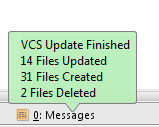
\includegraphics[width=0.4\linewidth]{../images/VCS}
		\caption{Integración de Git en Android Studio}
		\label{fig:VCS}
	\end{figure}

	Para ello decidimos utilizar \textbf{Git} y \textbf{GitHub}.
	Git es un sistema de control de versiones distribuido, con Git tenemos repositorios de software. GitHub es un servicio para hacer hosting de repositorios de software que se administra con Git. Digamos que en GitHub mantienes una copia de tus repositorios en la nube, que además puedes hacer disponible para otros desarrolladores\cite{gitexplicacion}.\\* 
	
	Posteriormente decidimos incluir también la propia memoria en GitHub, ya que otras soluciones de documentación en la nube nos convencían menos (De esto se hablará más adelante).\\*
	
	
	
	Al adoptar git, abrazamos este sistema con todas sus virtudes y sus defectos, al principio si ya has trabajado con otros sistemas de control de versiones, debes desechar estos conocimientos, ya que tienen que ver muy poco con el funcionamiento que tiene git a la hora de llevar el control sobre los archivos versionados.\\*
	
	Otros sistemas como podrían ser subversión, (utilizamos este ejemplo por ser bastante conocido) realizan copia de los archivos versionados cada vez que se cambia algo, sin embargo, el sistema de git, hace que sea más del estilo a una fotografía, donde se cambian los archivos nuevos o modificados pero sin embrago mantiene sin modificaciones los que no se han tocado, haciendo su uso bastante más eficiente\cite{funcgit2}.\\*
	
	\begin{figure}[H]
	\centering
	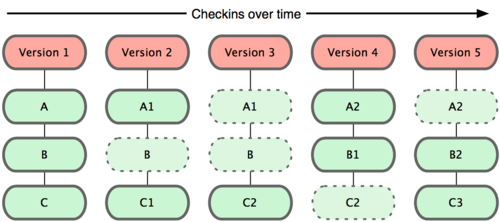
\includegraphics[width=0.7\linewidth]{../images/funcionamiento_git}
	\caption{Funcionamiento de git en el versionado}
	\label{fig:funcionamiento_git}
	\end{figure}


	\begin{figure}[H]
		\centering
		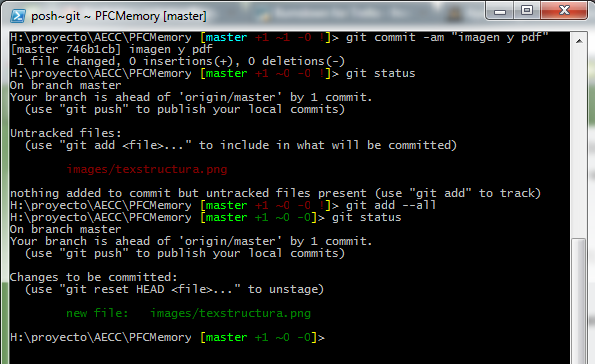
\includegraphics[width=0.7\linewidth]{../images/powershellcommit}
		\caption{PowerShell para windows}
		\label{fig:powershellcommit}
	\end{figure}
	


	\begin{figure}[H]
		\centering
		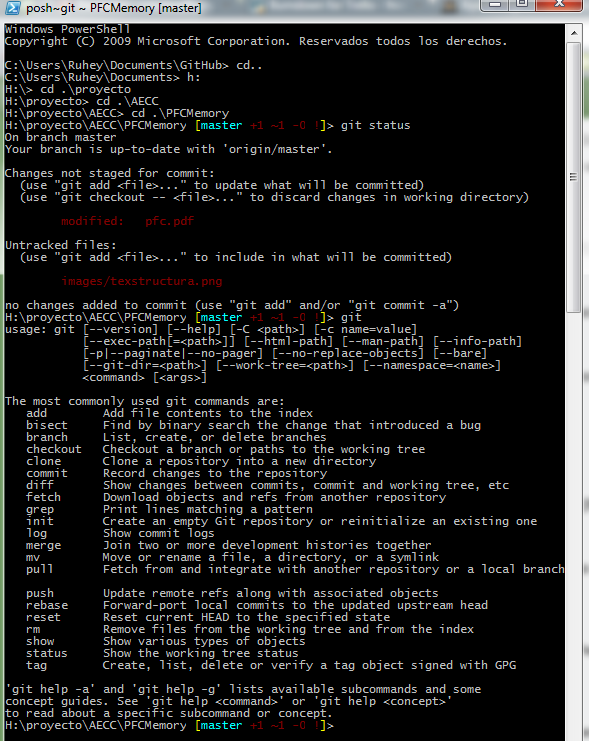
\includegraphics[width=0.7\linewidth]{../images/powerShell}
		\caption{PowerShell para windows}
		\label{fig:powershell}
	\end{figure}

	
	\begin{figure}[H]
		\centering
		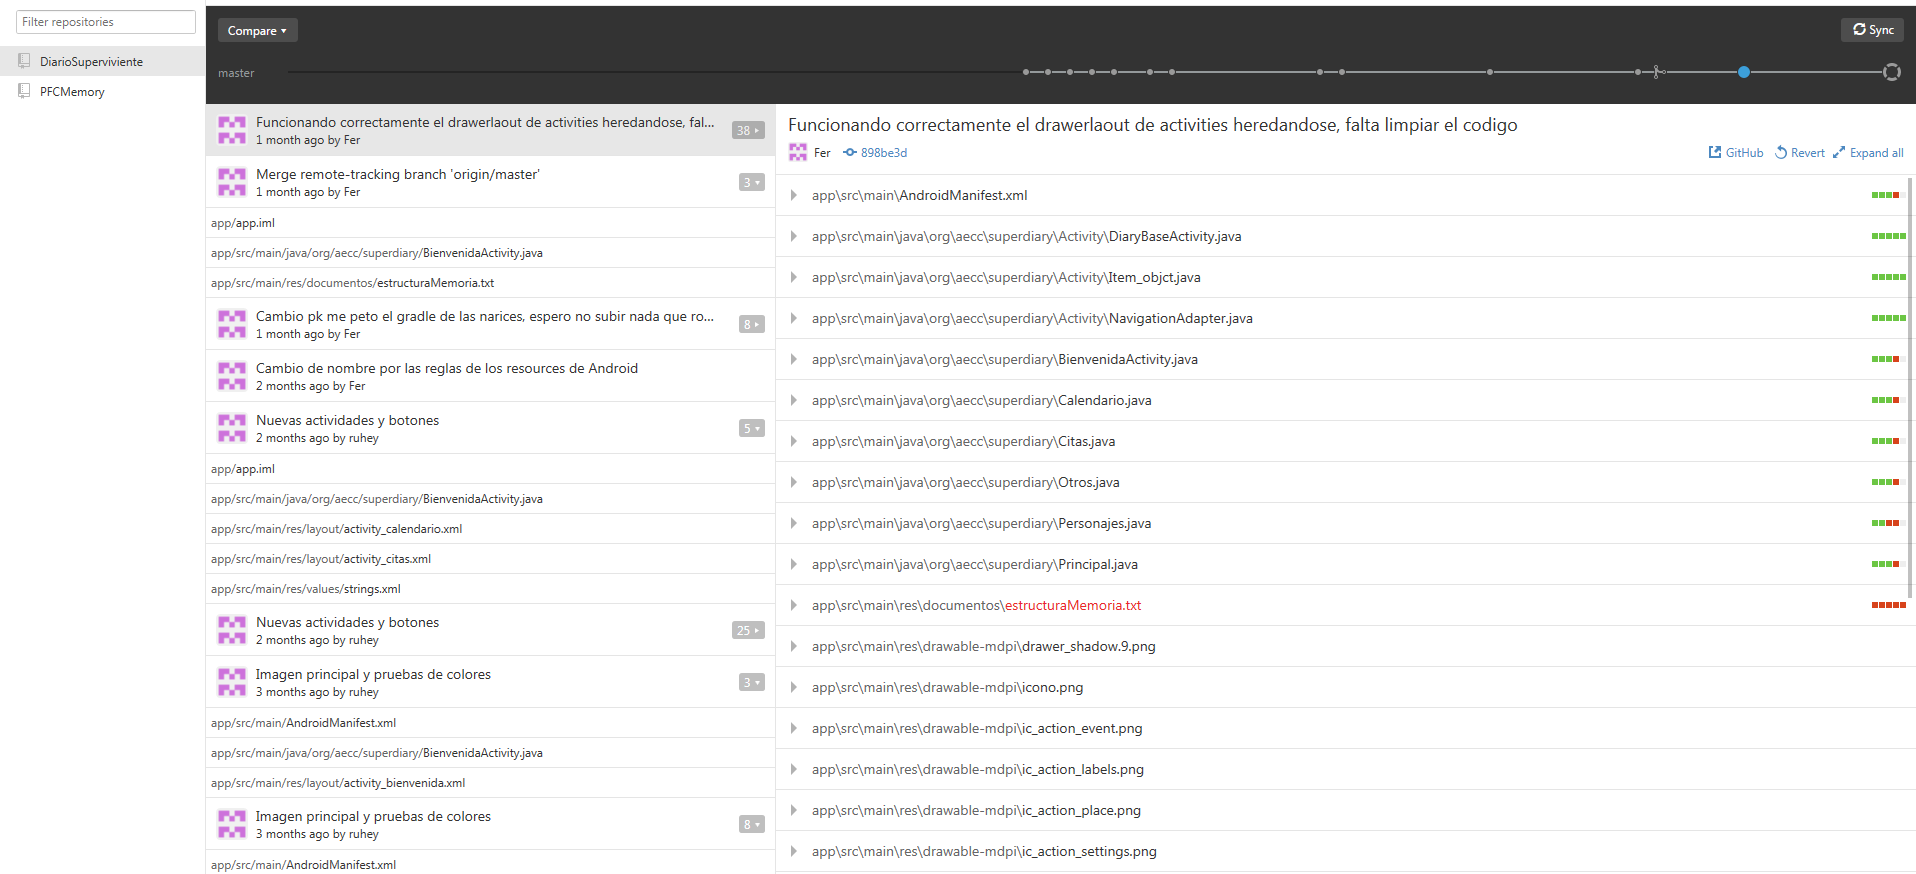
\includegraphics[width=1\linewidth]{../images/githubdesktopAplication}
		\caption{Github desktop, repositorio de la aplicación}
		\label{fig:ghdesktopA}
	\end{figure}

	
	\begin{figure}[H]
		\centering
		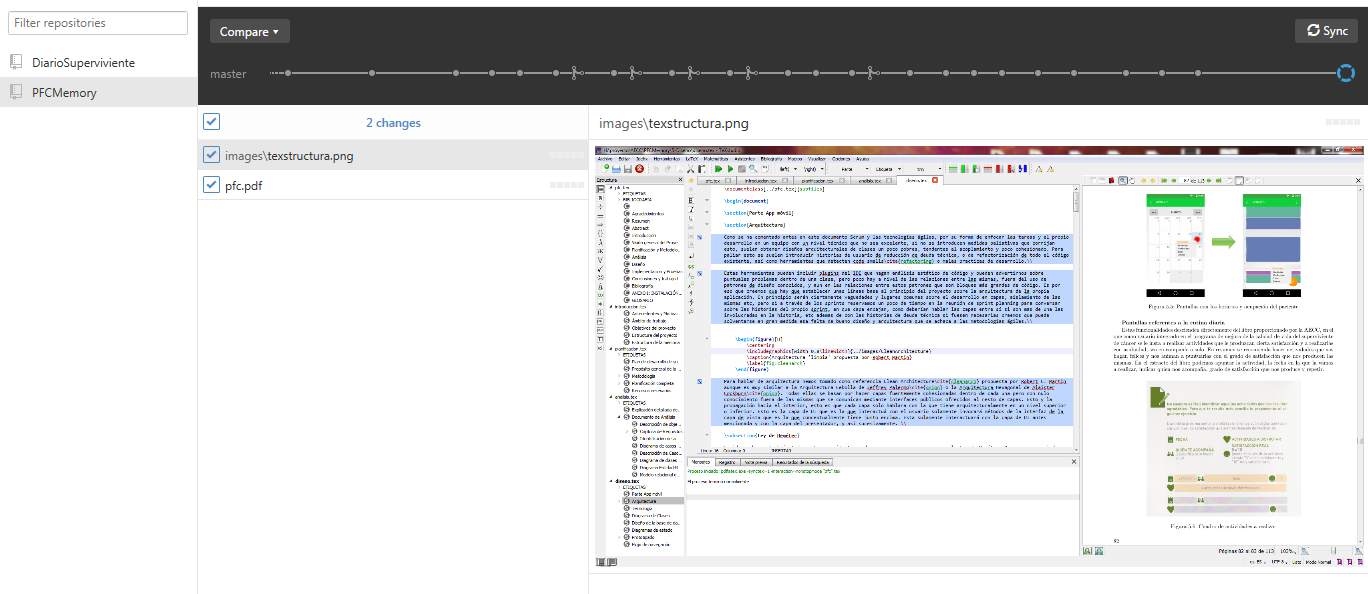
\includegraphics[width=1\linewidth]{../images/githubdesktopmemory}
		\caption{Github desktop, repositorio de la aplicación}
		\label{fig:ghdesktopM}
	\end{figure}

	
	\section{Plan de trabajo y comunicaciones}

	
	

	

	
	
	\section{Pruebas}
	
	\subsection{Plan de pruebas}
	
	\subsection{Tipos de pruebas}
		
	\subsection{Baterías de pruebas}
		
	\subsection{Pruebas en el dispositivo}
	
	\section{Puesta en producción}
	
\end{document}